\section{Présentation des données}
Comme dit précédemment, nous avons à dispositions plusieurs sets de
données en anglais et en français. Nous utiliserons uniquement les
sets de données en français.


Ces données sont sous forme de fichiers {\verb .json }, chaque
fichier correspond à un \emph{ dataset }, qui est un ensemble de
couples (phrase, labels), ou chaque label $\in$ labels correspond à la
nature grammatical du mot correspondant.


Pour chaque set de données, nous indiquons les informations suivantes: 
\begin{description}
\item[Présentation brève du dataset]
\item[Pourcentage des mots hors vocabulaire] Pourcentage de mots
  apparaissant uniquement dans les données de test, par rapport à
  l'ensemble du vocabulaire
\item[KL-Divergence] La divergence de Kullback-Leibler entre les
  données d'entraînement et de test
\item[Distribution des différents labels] dans le dataset
\item[Mots les plus utilisés] dans le dataset. 
\end{description}

\singlespacing
\clearpage \subsection{pud} 
 \begin{itemize} 
 \item[Présentation :] Phrases qui proviennent de sites informatifs, id est de journaux ou de Wikipedia

 \item[Pourcentage de mots hors vocabulaire : ]54.04
 \item[KL-Divergence :]0.256
 \end{itemize}  \subparagraph{Données de test \\ }  
 Nombre de phrases : 1000\\ 
\begin{figure}[H] \begin{minipage}{0.48\textwidth} \centering \begin{tabular}{|l || *{11 }{|c} |} \hline
Mot & Apparitions  \\ \hline
\begin{verb} , \end{verb} &1178\\ \hline
\begin{verb} de \end{verb} &1175\\ \hline
\begin{verb} . \end{verb} &985\\ \hline
\begin{verb} la \end{verb} &675\\ \hline
\begin{verb} et \end{verb} &442\\ \hline
\begin{verb} le \end{verb} &414\\ \hline
\begin{verb} les \end{verb} &399\\ \hline
\begin{verb} à \end{verb} &370\\ \hline
\begin{verb} l' \end{verb} &328\\ \hline
\begin{verb} des \end{verb} &327\\ \hline

\end{tabular}
\caption{ Mots les plus utilisés dans le set pud(test) } \label{Fig:muw}\end{minipage} 
\begin{minipage}{0.48\textwidth} \centering
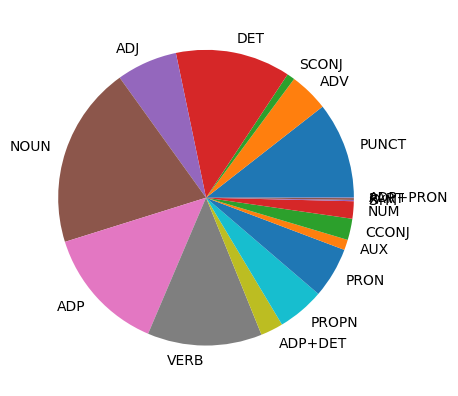
\includegraphics[width=.7\linewidth]{pudtest_img.png}
\caption{distribution des labels}
\end{minipage}
\end{figure} \subparagraph{Données de train \\ }  
 Nombre de phrases : 803\\ 
\begin{figure}[H] \begin{minipage}{0.48\textwidth} \centering \begin{tabular}{|l || *{11 }{|c} |} \hline
Mot & Apparitions  \\ \hline
\begin{verb} de \end{verb} &1114\\ \hline
\begin{verb} , \end{verb} &1016\\ \hline
\begin{verb} . \end{verb} &750\\ \hline
\begin{verb} la \end{verb} &683\\ \hline
\begin{verb} et \end{verb} &544\\ \hline
\begin{verb} l' \end{verb} &486\\ \hline
\begin{verb} des \end{verb} &432\\ \hline
\begin{verb} à \end{verb} &404\\ \hline
\begin{verb} d' \end{verb} &397\\ \hline
\begin{verb} le \end{verb} &385\\ \hline

\end{tabular}
\caption{ Mots les plus utilisés dans le set pud(train) } \label{Fig:muw}\end{minipage} 
\begin{minipage}{0.48\textwidth} \centering
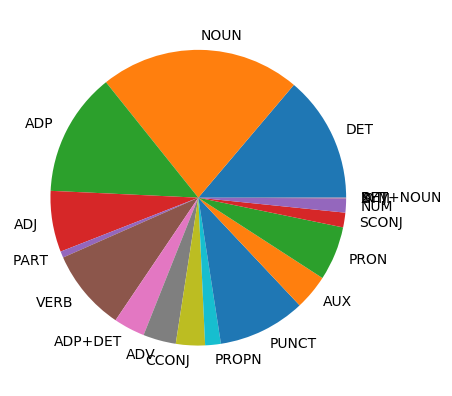
\includegraphics[width=.7\linewidth]{pudtrain_img.png}
\caption{distribution des labels}
\end{minipage}
\end{figure}


\clearpage \subsection{ftb } 
 \begin{itemize} 
 \item[Présentation :] Phrases provenant du journal «Le Monde»

 \item[Pourcentage de mots hors vocabulaire : ]7.099
 \item[KL-Divergence :]0.110
 \end{itemize}  \subparagraph{Données de test \\ }  
 Nombre de phrases : 2541\\ 
\begin{figure}[H] \begin{minipage}{0.48\textwidth} \centering \begin{tabular}{|l || *{11 }{|c} |} \hline
Mot & Apparitions  \\ \hline
\begin{verb} , \end{verb} &4528\\ \hline
\begin{verb} de \end{verb} &3593\\ \hline
\begin{verb} . \end{verb} &2258\\ \hline
\begin{verb} __DIGIT__ \end{verb} &2200\\ \hline
\begin{verb} la \end{verb} &2016\\ \hline
\begin{verb} l' \end{verb} &1350\\ \hline
\begin{verb} à \end{verb} &1333\\ \hline
\begin{verb} le \end{verb} &1293\\ \hline
\begin{verb} des \end{verb} &1255\\ \hline
\begin{verb} les \end{verb} &1222\\ \hline

\end{tabular}
\caption{ Mots les plus utilisés dans le set ftb(test) } \label{Fig:muw}\end{minipage} 
\begin{minipage}{0.48\textwidth} \centering
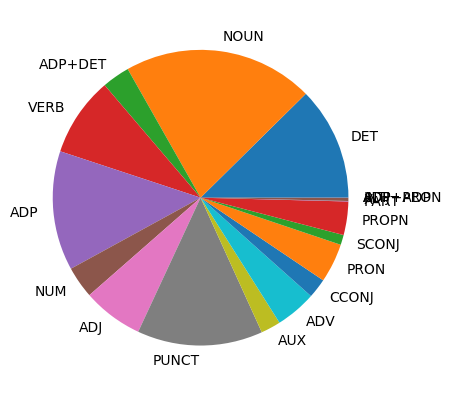
\includegraphics[width=.7\linewidth]{ftbtest_img.png}
\caption{distribution des labels}
\end{minipage}
\end{figure} \subparagraph{Données de train \\ }  
 Nombre de phrases : 14759\\ 
\begin{figure}[H] \begin{minipage}{0.48\textwidth} \centering \begin{tabular}{|l || *{11 }{|c} |} \hline
Mot & Apparitions  \\ \hline
\begin{verb} , \end{verb} &27318\\ \hline
\begin{verb} de \end{verb} &22518\\ \hline
\begin{verb} . \end{verb} &13735\\ \hline
\begin{verb} __DIGIT__ \end{verb} &11104\\ \hline
\begin{verb} la \end{verb} &10780\\ \hline
\begin{verb} l' \end{verb} &8129\\ \hline
\begin{verb} à \end{verb} &7984\\ \hline
\begin{verb} le \end{verb} &7255\\ \hline
\begin{verb} les \end{verb} &7086\\ \hline
\begin{verb} des \end{verb} &7071\\ \hline

\end{tabular}
\caption{ Mots les plus utilisés dans le set ftb(train) } \label{Fig:muw}\end{minipage} 
\begin{minipage}{0.48\textwidth} \centering
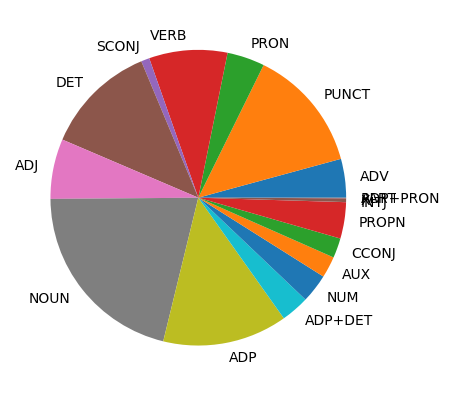
\includegraphics[width=.7\linewidth]{ftbtrain_img.png}
\caption{distribution des labels}
\end{minipage}
\end{figure}


\clearpage \subsection{spoken } 
 \begin{itemize} 
 \item[Présentation :] Données sur le français oral

 \item[Pourcentage de mots hors vocabulaire : ]32.14
 \item[KL-Divergence :]0.366
 \end{itemize}  \subparagraph{Données de test \\ }  
 Nombre de phrases : 726\\ 
\begin{figure}[H] \begin{minipage}{0.48\textwidth} \centering \begin{tabular}{|l || *{11 }{|c} |} \hline
Mot & Apparitions  \\ \hline
\begin{verb} de \end{verb} &380\\ \hline
\begin{verb} est \end{verb} &262\\ \hline
\begin{verb} euh \end{verb} &222\\ \hline
\begin{verb} la \end{verb} &219\\ \hline
\begin{verb} et \end{verb} &193\\ \hline
\begin{verb} que \end{verb} &188\\ \hline
\begin{verb} le \end{verb} &181\\ \hline
\begin{verb} l' \end{verb} &177\\ \hline
\begin{verb} à \end{verb} &169\\ \hline
\begin{verb} je \end{verb} &162\\ \hline

\end{tabular}
\caption{ Mots les plus utilisés dans le set spoken(test) } \label{Fig:muw}\end{minipage} 
\begin{minipage}{0.48\textwidth} \centering
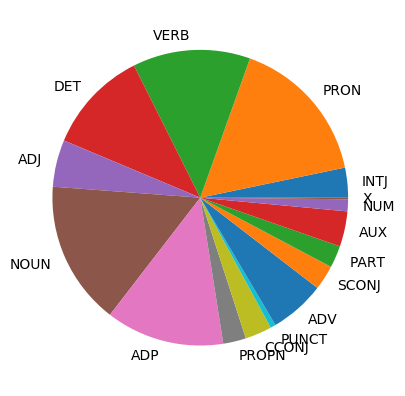
\includegraphics[width=.7\linewidth]{spokentest_img.png}
\caption{distribution des labels}
\end{minipage}
\end{figure} \subparagraph{Données de train \\ }  
 Nombre de phrases : 1153\\ 
\begin{figure}[H] \begin{minipage}{0.48\textwidth} \centering \begin{tabular}{|l || *{11 }{|c} |} \hline
Mot & Apparitions  \\ \hline
\begin{verb} de \end{verb} &529\\ \hline
\begin{verb} euh \end{verb} &489\\ \hline
\begin{verb} est \end{verb} &362\\ \hline
\begin{verb} la \end{verb} &339\\ \hline
\begin{verb} et \end{verb} &328\\ \hline
\begin{verb} le \end{verb} &294\\ \hline
\begin{verb} à \end{verb} &282\\ \hline
\begin{verb} c' \end{verb} &264\\ \hline
\begin{verb} je \end{verb} &223\\ \hline
\begin{verb} qui \end{verb} &218\\ \hline

\end{tabular}
\caption{ Mots les plus utilisés dans le set spoken(train) } \label{Fig:muw}\end{minipage} 
\begin{minipage}{0.48\textwidth} \centering
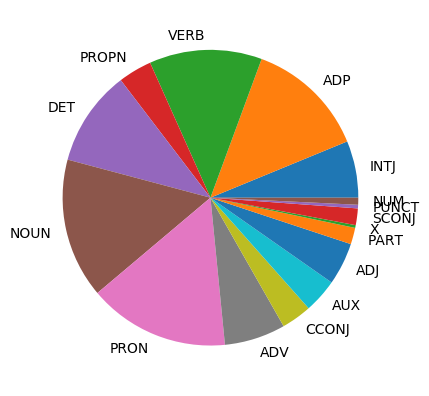
\includegraphics[width=.7\linewidth]{spokentrain_img.png}
\caption{distribution des labels}
\end{minipage}
\end{figure}


\clearpage \subsection{sequoia } 
 \begin{itemize} 
 \item[Présentation :] Ensemble de texte, à la base disponible avec des annotations «profondes», ie plus complètes. Néanmoins, ces annotations ont été normalisées par rapport aux autres données

 \item[Pourcentage de mots hors vocabulaire : ]9.417
 \item[KL-Divergence :]0.113
 \end{itemize}  \subparagraph{Données de test \\ }  
 Nombre de phrases : 456\\ 
\begin{figure}[H] \begin{minipage}{0.48\textwidth} \centering \begin{tabular}{|l || *{11 }{|c} |} \hline
Mot & Apparitions  \\ \hline
\begin{verb} de \end{verb} &463\\ \hline
\begin{verb} , \end{verb} &431\\ \hline
\begin{verb} . \end{verb} &344\\ \hline
\begin{verb} la \end{verb} &216\\ \hline
\begin{verb} __DIGIT__ \end{verb} &204\\ \hline
\begin{verb} l' \end{verb} &186\\ \hline
\begin{verb} à \end{verb} &169\\ \hline
\begin{verb} et \end{verb} &165\\ \hline
\begin{verb} des \end{verb} &152\\ \hline
\begin{verb} d' \end{verb} &139\\ \hline

\end{tabular}
\caption{ Mots les plus utilisés dans le set sequoia(test) } \label{Fig:muw}\end{minipage} 
\begin{minipage}{0.48\textwidth} \centering
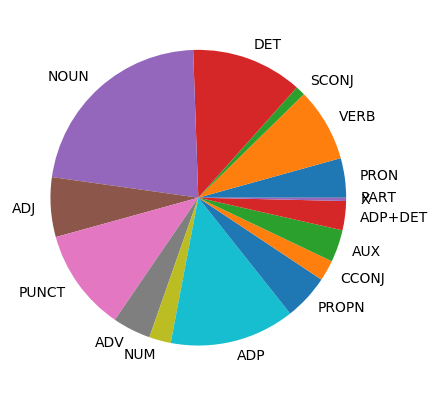
\includegraphics[width=.7\linewidth]{sequoiatest_img.png}
\caption{distribution des labels}
\end{minipage}
\end{figure} \subparagraph{Données de train \\ }  
 Nombre de phrases : 2231\\ 
\begin{figure}[H] \begin{minipage}{0.48\textwidth} \centering \begin{tabular}{|l || *{11 }{|c} |} \hline
Mot & Apparitions  \\ \hline
\begin{verb} de \end{verb} &2435\\ \hline
\begin{verb} , \end{verb} &2354\\ \hline
\begin{verb} . \end{verb} &1683\\ \hline
\begin{verb} la \end{verb} &1176\\ \hline
\begin{verb} __DIGIT__ \end{verb} &1039\\ \hline
\begin{verb} l' \end{verb} &916\\ \hline
\begin{verb} à \end{verb} &857\\ \hline
\begin{verb} et \end{verb} &845\\ \hline
\begin{verb} des \end{verb} &759\\ \hline
\begin{verb} le \end{verb} &743\\ \hline

\end{tabular}
\caption{ Mots les plus utilisés dans le set sequoia(train) } \label{Fig:muw}\end{minipage} 
\begin{minipage}{0.48\textwidth} \centering
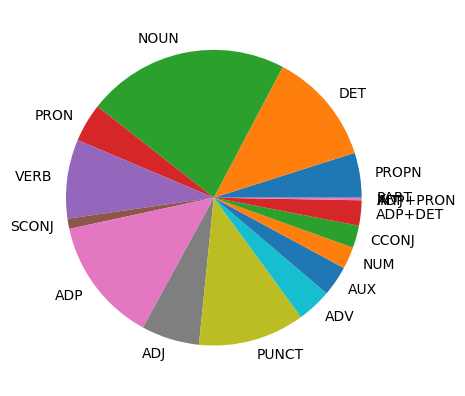
\includegraphics[width=.7\linewidth]{sequoiatrain_img.png}
\caption{distribution des labels}
\end{minipage}
\end{figure}


\clearpage \subsection{partut } 
 \begin{itemize} 
 \item[Présentation :] Ensemble varié de textes, incluant de extraits de conférences comme des extraits de Wikipedia ou des textes légaux

 \item[Pourcentage de mots hors vocabulaire : ]5.743
 \item[KL-Divergence :]0.330
 \end{itemize}  \subparagraph{Données de test \\ }  
 Nombre de phrases : 110\\ 
\begin{figure}[H] \begin{minipage}{0.48\textwidth} \centering \begin{tabular}{|l || *{11 }{|c} |} \hline
Mot & Apparitions  \\ \hline
\begin{verb} de \end{verb} &120\\ \hline
\begin{verb} . \end{verb} &110\\ \hline
\begin{verb} , \end{verb} &79\\ \hline
\begin{verb} la \end{verb} &69\\ \hline
\begin{verb} à \end{verb} &58\\ \hline
\begin{verb} l' \end{verb} &56\\ \hline
\begin{verb} les \end{verb} &46\\ \hline
\begin{verb} et \end{verb} &42\\ \hline
\begin{verb} des \end{verb} &39\\ \hline
\begin{verb} le \end{verb} &39\\ \hline

\end{tabular}
\caption{ Mots les plus utilisés dans le set partut(test) } \label{Fig:muw}\end{minipage} 
\begin{minipage}{0.48\textwidth} \centering
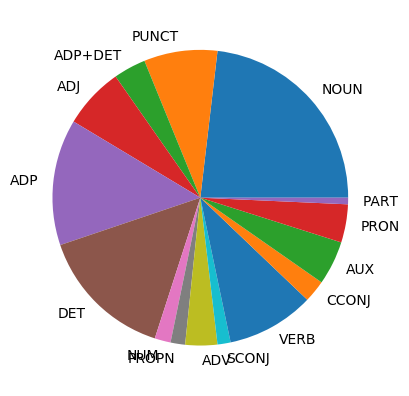
\includegraphics[width=.7\linewidth]{partuttest_img.png}
\caption{distribution des labels}
\end{minipage}
\end{figure} \subparagraph{Données de train \\ }  
 Nombre de phrases : 803\\ 
\begin{figure}[H] \begin{minipage}{0.48\textwidth} \centering \begin{tabular}{|l || *{11 }{|c} |} \hline
Mot & Apparitions  \\ \hline
\begin{verb} de \end{verb} &1114\\ \hline
\begin{verb} , \end{verb} &1016\\ \hline
\begin{verb} . \end{verb} &750\\ \hline
\begin{verb} la \end{verb} &683\\ \hline
\begin{verb} et \end{verb} &544\\ \hline
\begin{verb} l' \end{verb} &486\\ \hline
\begin{verb} des \end{verb} &432\\ \hline
\begin{verb} à \end{verb} &404\\ \hline
\begin{verb} d' \end{verb} &397\\ \hline
\begin{verb} le \end{verb} &385\\ \hline

\end{tabular}
\caption{ Mots les plus utilisés dans le set partut(train) } \label{Fig:muw}\end{minipage} 
\begin{minipage}{0.48\textwidth} \centering
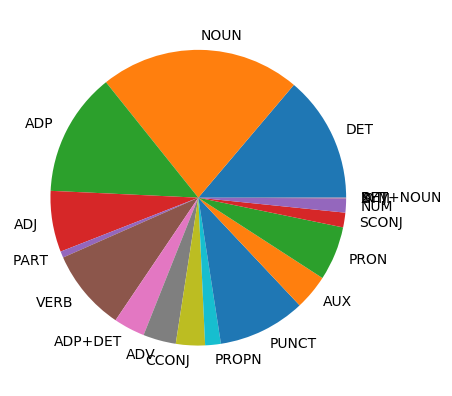
\includegraphics[width=.7\linewidth]{partuttrain_img.png}
\caption{distribution des labels}
\end{minipage}
\end{figure}


\clearpage \subsection{gsd } 
 \begin{itemize} 
 \item[Présentation :] Phrases variées

 \item[Pourcentage de mots hors vocabulaire : ]1.359
 \item[KL-Divergence :]0.409
 \end{itemize}  \subparagraph{Données de test \\ }  
 Nombre de phrases : 416\\ 
\begin{figure}[H] \begin{minipage}{0.48\textwidth} \centering \begin{tabular}{|l || *{11 }{|c} |} \hline
Mot & Apparitions  \\ \hline
\begin{verb} , \end{verb} &489\\ \hline
\begin{verb} de \end{verb} &426\\ \hline
\begin{verb} . \end{verb} &353\\ \hline
\begin{verb} la \end{verb} &222\\ \hline
\begin{verb} et \end{verb} &182\\ \hline
\begin{verb} l' \end{verb} &171\\ \hline
\begin{verb} à \end{verb} &168\\ \hline
\begin{verb} __DIGIT__ \end{verb} &166\\ \hline
\begin{verb} le \end{verb} &155\\ \hline
\begin{verb} les \end{verb} &127\\ \hline

\end{tabular}
\caption{ Mots les plus utilisés dans le set gsd(test) } \label{Fig:muw}\end{minipage} 
\begin{minipage}{0.48\textwidth} \centering
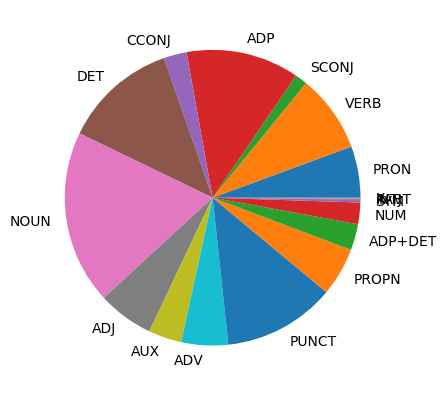
\includegraphics[width=.7\linewidth]{gsdtest_img.png}
\caption{distribution des labels}
\end{minipage}
\end{figure} \subparagraph{Données de train \\ }  
 Nombre de phrases : 14450\\ 
\begin{figure}[H] \begin{minipage}{0.48\textwidth} \centering \begin{tabular}{|l || *{11 }{|c} |} \hline
Mot & Apparitions  \\ \hline
\begin{verb} de \end{verb} &16964\\ \hline
\begin{verb} , \end{verb} &16595\\ \hline
\begin{verb} . \end{verb} &13359\\ \hline
\begin{verb} la \end{verb} &8676\\ \hline
\begin{verb} et \end{verb} &7148\\ \hline
\begin{verb} __DIGIT__ \end{verb} &7095\\ \hline
\begin{verb} le \end{verb} &6389\\ \hline
\begin{verb} à \end{verb} &6216\\ \hline
\begin{verb} l' \end{verb} &5864\\ \hline
\begin{verb} en \end{verb} &4793\\ \hline

\end{tabular}
\caption{ Mots les plus utilisés dans le set gsd(train) } \label{Fig:muw}\end{minipage} 
\begin{minipage}{0.48\textwidth} \centering
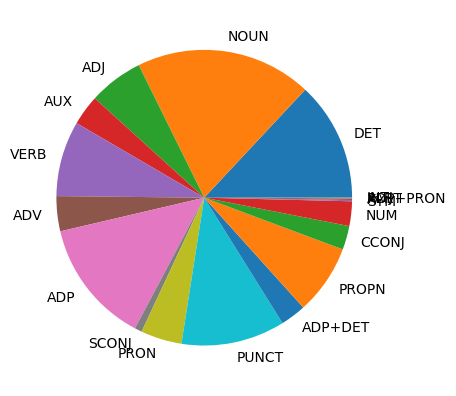
\includegraphics[width=.7\linewidth]{gsdtrain_img.png}
\caption{distribution des labels}
\end{minipage}
\end{figure}

\clearpage
\subsection{foot } 
 \begin{itemize} 
 \item[Présentation :] Ensemble de tweets parlant de football

 \end{itemize}  \subparagraph{Données de test \\ }  
 Nombre de phrases : 743\\ 
\begin{figure}[H] \begin{minipage}{0.48\textwidth} \centering \begin{tabular}{|l || *{11 }{|c} |} \hline
Mot & Apparitions  \\ \hline
\begin{verb} __MENTION__ \end{verb} &549\\ \hline
\begin{verb} la \end{verb} &433\\ \hline
\begin{verb} __SHARP__ \end{verb} &395\\ \hline
\begin{verb} Juventus \end{verb} &368\\ \hline
\begin{verb} : \end{verb} &338\\ \hline
\begin{verb} de \end{verb} &325\\ \hline
\begin{verb} ! \end{verb} &314\\ \hline
\begin{verb} le \end{verb} &257\\ \hline
\begin{verb} , \end{verb} &247\\ \hline
\begin{verb} __URL__ \end{verb} &226\\ \hline

\end{tabular}
\caption{ Mots les plus utilisés dans le set foot(test) } \label{Fig:muw}\end{minipage} 
\begin{minipage}{0.48\textwidth} \centering
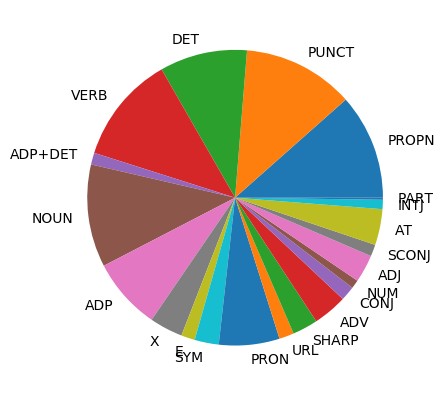
\includegraphics[width=.7\linewidth]{foottest_img.png}
\caption{distribution des labels}
\end{minipage}
\end{figure}


 \subsection{natdis } 
 \begin{itemize} 
 \item[Présentation :] Ensemble de tweets

 \end{itemize}  \subparagraph{Données de test \\ }  
 Nombre de phrases : 622\\ 
\begin{figure}[H] \begin{minipage}{0.48\textwidth} \centering \begin{tabular}{|l || *{11 }{|c} |} \hline
Mot & Apparitions  \\ \hline
\begin{verb} de \end{verb} &994\\ \hline
\begin{verb} __URL__ \end{verb} &469\\ \hline
\begin{verb} __DIGIT__ \end{verb} &411\\ \hline
\begin{verb} terre \end{verb} &338\\ \hline
\begin{verb} __SHARP__ \end{verb} &300\\ \hline
\begin{verb} tremblement \end{verb} &295\\ \hline
\begin{verb} : \end{verb} &285\\ \hline
\begin{verb} chaleur \end{verb} &244\\ \hline
\begin{verb} au \end{verb} &220\\ \hline
\begin{verb} vague \end{verb} &206\\ \hline

\end{tabular}
\caption{ Mots les plus utilisés dans le set natdis(test) } \label{Fig:muw}\end{minipage} 
\begin{minipage}{0.48\textwidth} \centering
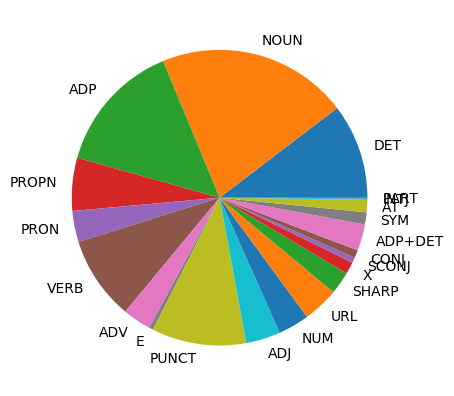
\includegraphics[width=.7\linewidth]{natdistest_img.png}
\caption{distribution des labels}
\end{minipage}
\end{figure}

\onehalfspacing

